\section{Zusätzliche Bewegungsabläufe}
\subsection{Anforderungen}
Dieses Kapitel beschäftigt sich mit den Einschränkungen der Walker-Demonstration im Bezug auf unterschiedliche Bewegungabläufe. Das trainierte Modell der Walker Demo beherrscht nur die Fortbewegung in Blickrichtung. Der Läufer ist auch nicht darauf trainiert stehen zu bleiben. Das resultiert darin, dass der Läufer fällt sobald der Nutzer keinen Tastaturinput gibt. Es werden Anpassungen am Trainingsablauf getestet um den Läufer darauf zu trainieren unabhängig von der Bewegungsrichtung eine zusätzliche Blickrichtung zu halten, sowie auf der stelle zu stehen. 

\subsection{360 Grad Blickziel}
Der ersten Versuch eine separate Blickrichtung dem Training hinzuzufügen, wurde von den Methoden der Walker Demo inspiriert. Gleich wie das Laufziel wurde ein zusätzliches Zielobjekt hinzugefügt, welches zufällig platziert wurde. Um die Komplexität nicht von Anfang an zu hoch anzusetzen, wurde das Blickziel zu beginn die Winkelabweichung zwischen Zielrichtung und Blickrichtung langsam über ein Lehrplan angepasst. Anfangs wurde das Blickziel mit einer Winkelabweichung im Bereich von -5 und 5 Grad platziert, zum Ende hin wurde der Bereich immer weiter bis auf -90 bis 90 Grad erweitert (siehe Codeausschnitt \ref{lst:lehrplan_blickziel}). Das Blickziel wurde neu gesetzt sobald ein Ziel erreicht wurde.

\begin{lstlisting}[caption={ Lehrplan für das Blickziel},captionpos=b,label={lst:lehrplan_blickziel}]
lookAngleLimit:
    curriculum:
      - name: min max 5 degree look target deviation
        completion_criteria:
          measure: progress
          behavior: Walker
          threshold: 0.4
          signal_smoothing: true
        value: 5.0
      - name: min max 30 degree look target deviation
        completion_criteria:
          measure: progress
          behavior: Walker
          threshold: 0.6
          signal_smoothing: true
          require_reset: true
        value: 30.0
      - name: min max 60 degree look target deviation
        completion_criteria:
          measure: progress
          behavior: Walker
          threshold: 0.8
          signal_smoothing: true
          require_reset: true
        value: 60.0
      - name: min max 90 degree look target deviation
        completion_criteria:
          measure: progress
          behavior: Walker
          threshold: 1.0
          signal_smoothing: true
          require_reset: true
        value: 90.0
\end{lstlisting}

Der Läufer lernt einen stabilen Gang (siehe Abbildungen \ref{fig:103_move_target_dir} und \ref{fig:103_reach_target}). Die Winkelabweichung von 5 Grad ist mit aktueller Belohnungsfunktion jedoch nahezu zu vernachlässigen. Vor folgenden Lehreinheiten hat sich bereits ein Verhalten so start gefestigt, das die Lehreinheiten keine Wirkung zeigen (siehe Abbildungen \ref{fig:103_look_angle_limit} und \ref{fig:126_look_reward}.

\begin{figure}[H]
  \centering  
    \begin{subfigure}{.49\textwidth}
      \centering  
      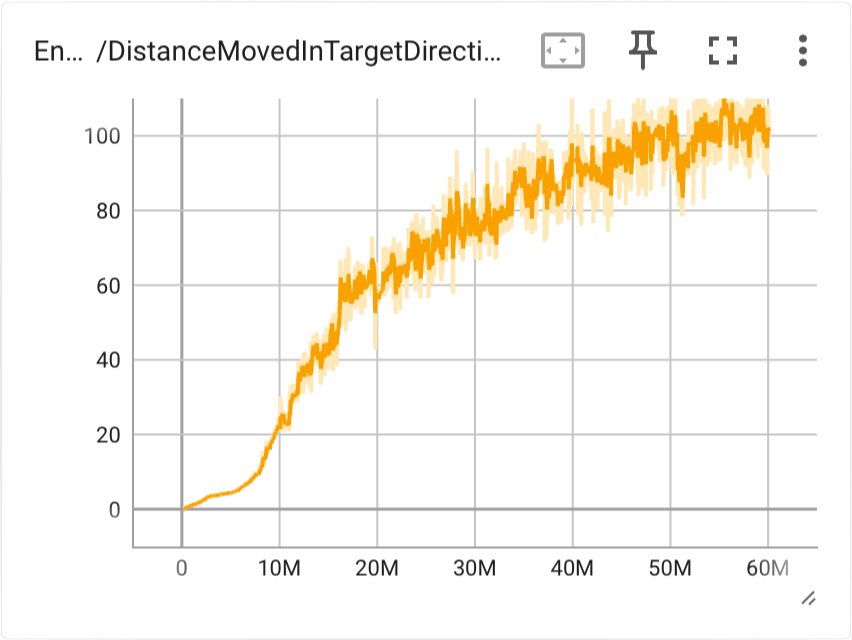
\includegraphics[width=\textwidth]{img/103_move_target_dir}
      \caption{Zurückgelegte Strecke in Zielrichtung}
      \label{fig:103_move_target_dir}
    \end{subfigure}
    \begin{subfigure}{.49\textwidth}
      \centering  
      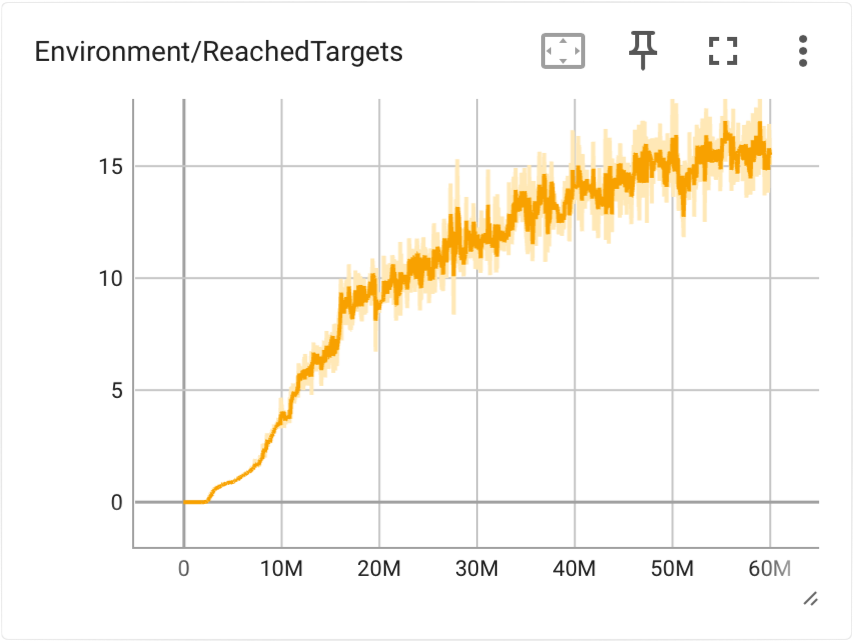
\includegraphics[width=\textwidth]{img/103_reach_target}
      \caption{Erreichte Anzahl an Zielen}
      \label{fig:103_reach_target}
    \end{subfigure}
    \begin{subfigure}{.49\textwidth}
      \centering  
      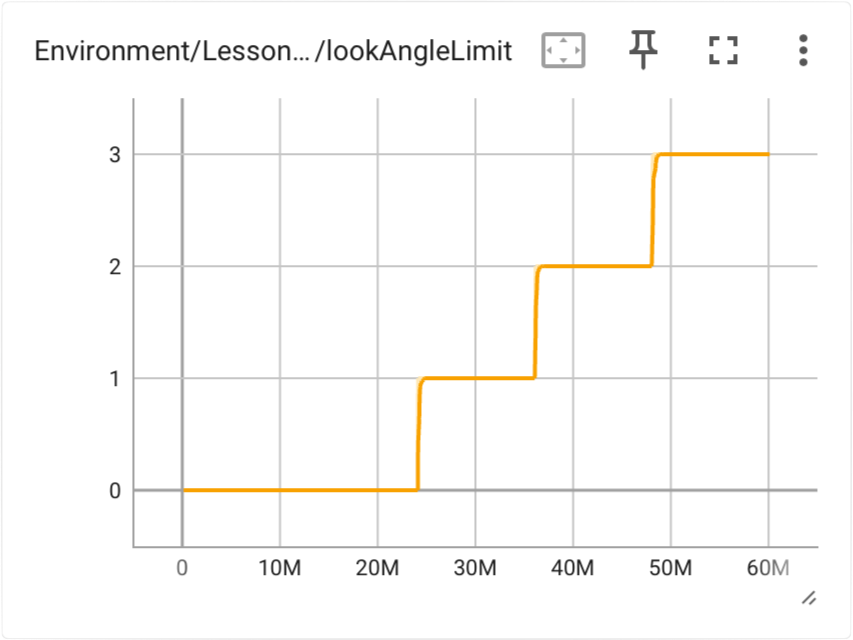
\includegraphics[width=\textwidth]{img/103_look_angle_limit}
      \caption{Aktive Lehreinheit}
      \label{fig:103_look_angle_limit}
    \end{subfigure}
     \begin{subfigure}{.49\textwidth}
      \centering  
      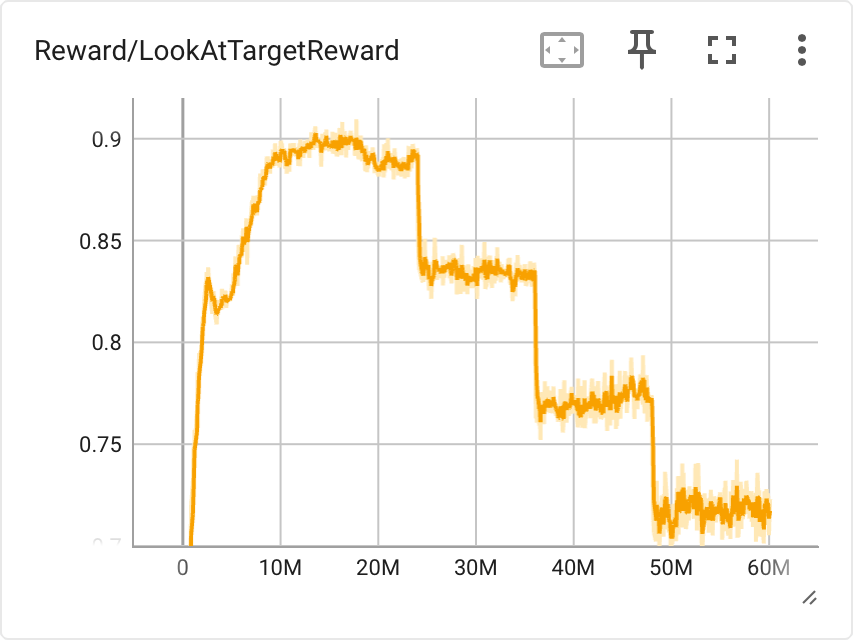
\includegraphics[width=\textwidth]{img/103_look_reward}
      \caption{Blickbelohnung}
      \label{fig:103_look_reward}
    \end{subfigure}
  \caption{Training Blickrichtungsziel mit Lehrplan}
  \label{fig:training_blickrichtungsziel_lehrplan}
\end{figure}

Um von Beginn an ein generell gültiges Verhalten anzutrainieren, wurden Trainings ohne Lehrplan durchgeführt. Dabei wurde ein Training mit einer Winkelabweichung von +-90 Grad und eins mit +-180 Grad durchgeführt. Der Läufer lernt bei beiden Trainings kaum die Blickrichtung der neuen Zielblickrichtung anzupassen. Bei Training mit Winkelabweichungen von bis zu +-180 Grad lernt der Läufer negative Belohnungen mit einer Blickrichtung vertikal nach unten zu umgehen. Dies ist möglich da die die Blickrichtung Vertikal nach unten entlang der Y-Achse verläuft. Bei der Berechnung der Blickbelohnung wird die Y-Komponente der Blickrichtung auf 0 gesetzt, da die Zielrichtung auch ohne Höhenkomponente festgelegt wird um Höhenunterschiede zwischen Hüfte und Ziel zu ignorieren. Durch dieses Schlupfloch kann der Läufer negative Belohnungen verhindern ohne die Gangart nennenswert anzupassen.

\begin{figure}[H]
  \centering  
    \begin{subfigure}{.49\textwidth}
      \centering  
      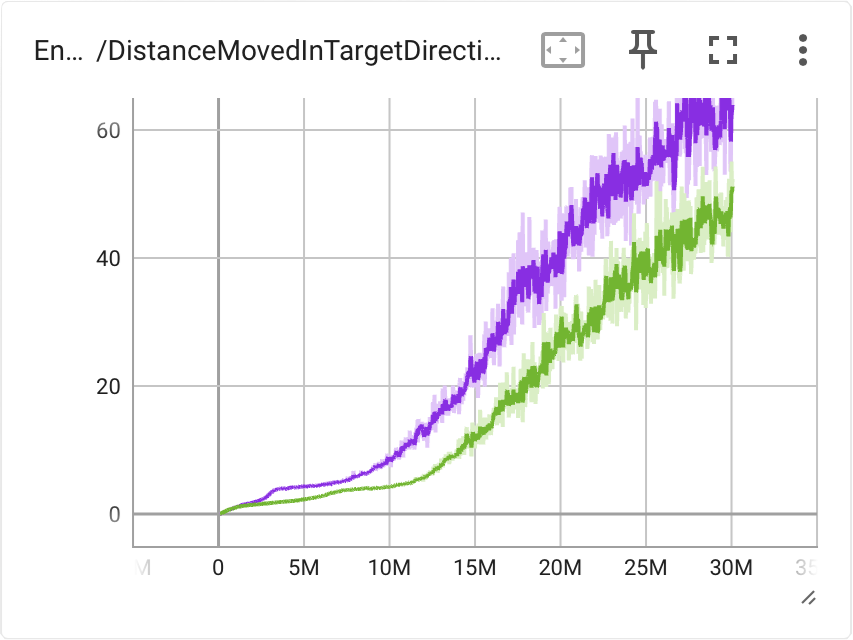
\includegraphics[width=\textwidth]{img/104_105_move_target_dir}
      \caption{Zurückgelegte Strecke in Zielrichtung}
      \label{fig:104_105_move_target_dir}
    \end{subfigure}
    \begin{subfigure}{.49\textwidth}
      \centering  
      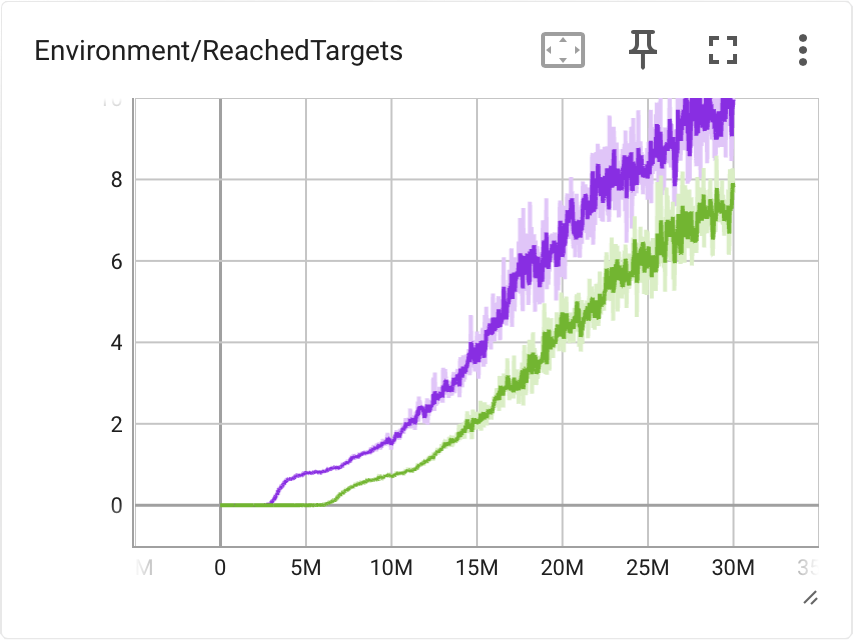
\includegraphics[width=\textwidth]{img/104_105_reach_target}
      \caption{Erreichte Anzahl an Zielen}
      \label{fig:104_105_reach_target}
    \end{subfigure}
    \begin{subfigure}{.49\textwidth}
      \centering  
      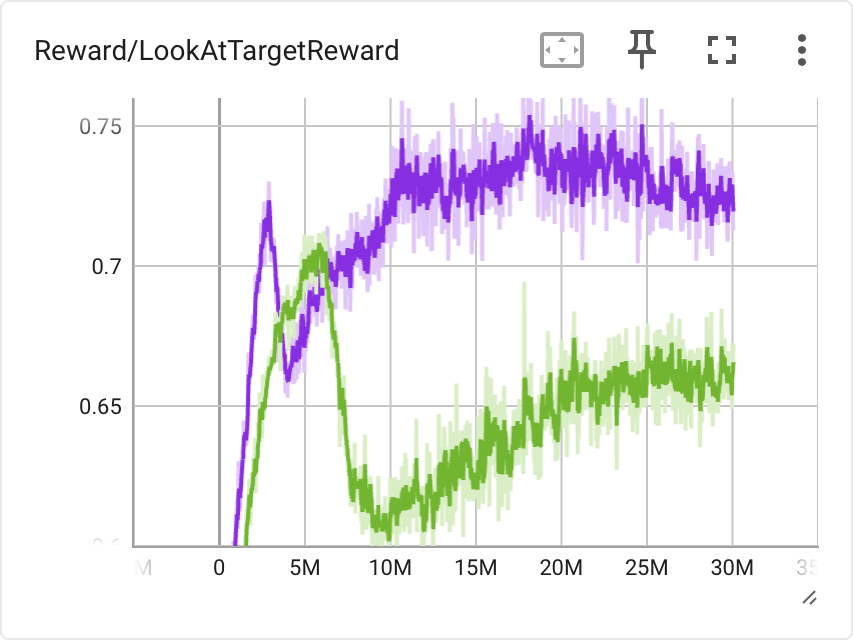
\includegraphics[width=\textwidth]{img/104_105_look_reward}
      \caption{Blickbelohnung}
      \label{fig:104_105_look_reward}
    \end{subfigure}
  \caption{Training Blickrichtungsziel (blau = Winkelabweichung +-90 Grad, grün = Winkelabweichung +-180 Grad)}
  \label{fig:training_blickrichtungsziel}
\end{figure}

Um das Schlupfloch der Blickbelohnung zu stopfen wird eine neue Bestrafung eingeführt. Die Kopfneigungsbestrafung bestraft den Läufer für das neigen des Kopfs und sorgt somit dafür das der Läufer den Kopf aufrecht hält. Im Training mit der neuen Kopfneigungsbestrafung lernt der Läufer langsamer und findet eine neuen Ausweg die Belohnungen generell gültig zu optimieren ohne unterschiedliche Gangarten zu erlernen. Durch die Eigenschaft des Trainings, dass der Winkel zwischen Läufer, Ziel und Blickziel nur bei der Platzierung des Blickziels eingehalten werden, werden die Winkel durch das annähern des Läufers zum Ziel ausnahmslos größer. Somit ist die beste Lösung für den Läufer sich rückwärts zu bewegen, denn so ist die Wahrscheinlichkeit das die Winkelabweichung kleiner ist wesentlich höher (siehe Abbildung \ref{fig:blickwinkel_änderung}).

\begin{figure}[H]
  \centering  
    \begin{subfigure}{.3\textwidth}
      \centering  
      \includegraphics[width=\textwidth]{img/blickwinkel_änderung1}
    \end{subfigure}
    \begin{subfigure}{.3\textwidth}
      \centering  
      \includegraphics[width=\textwidth]{img/blickwinkel_änderung2}
    \end{subfigure}
    \begin{subfigure}{.3\textwidth}
      \centering  
      \includegraphics[width=\textwidth]{img/blickwinkel_änderung3}
    \end{subfigure}
  \caption{Blickwinkel Änderung durch Zielannäherung}
  \label{fig:blickwinkel_änderung}
\end{figure}

Das Problem wurde behoben, indem das Blickziel in nachfolgenden Trainings kontinuierlich mit jedem Update neu platziert wurde, um somit den Blickwinkel gleich zu halten. In den bisherigen Trainingseinheiten hat der Läufer zudem eine Gangart optimiert um allen Blickziele mittelmäßig zu erreichen. Um den Läufer zu motivieren alle Blickziele stärker einzuhalten, wurde die Implementierung geändert, sodass der Blickwinkel beim erreichen des Laufziels nur noch gewechselt wird wenn die Durchschnittliche Blickbelohnung über dem Schwellenwert von 0.7 liegt. Mit dieser neuen Bedingung beim erreichen des Blickziels, erreicht der Läufer die ersten Blickziele und stagniert dann an den neuen Blickzielen (siehe \ref{fig:training_blickrichtungsziel_wechsel_07}).

\begin{figure}[H]
  \centering  
    \begin{subfigure}{.49\textwidth}
      \centering  
      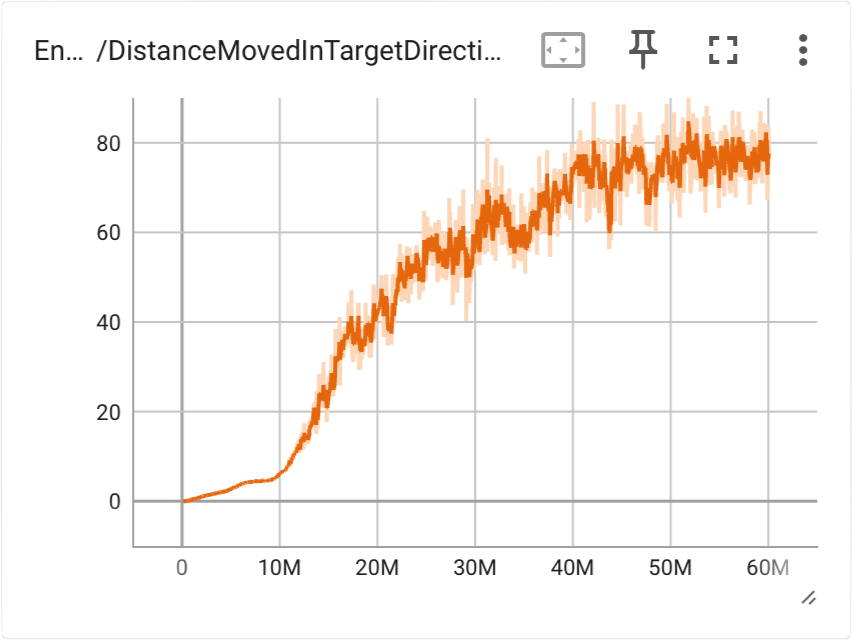
\includegraphics[width=\textwidth]{img/113_move_target_dir}
      \caption{Zurückgelegte Strecke in Zielrichtung}
      \label{fig:113_move_target_dir}
    \end{subfigure}
    \begin{subfigure}{.49\textwidth}
      \centering  
      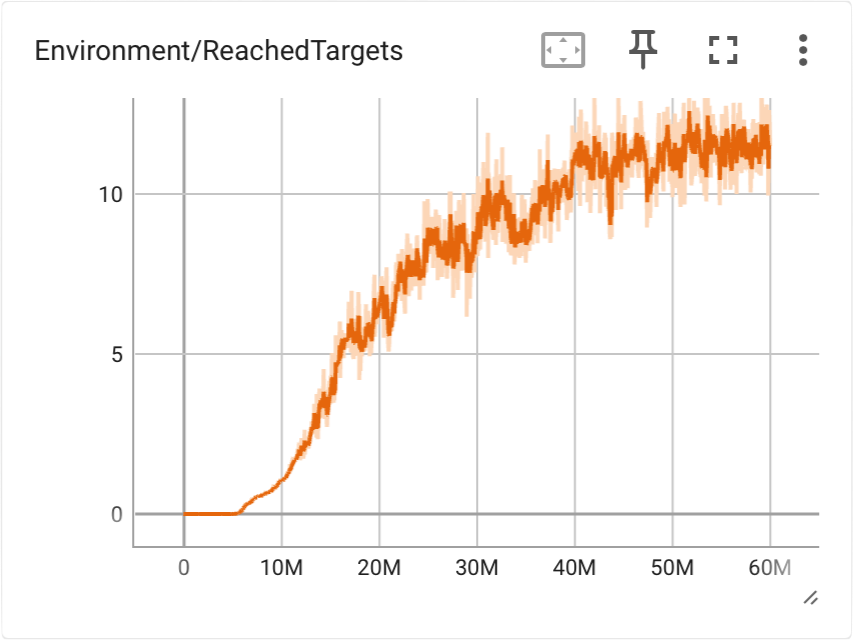
\includegraphics[width=\textwidth]{img/113_reach_target}
      \caption{Erreichte Anzahl an Zielen}
      \label{fig:113_reach_target}
    \end{subfigure}
    \begin{subfigure}{.49\textwidth}
      \centering  
      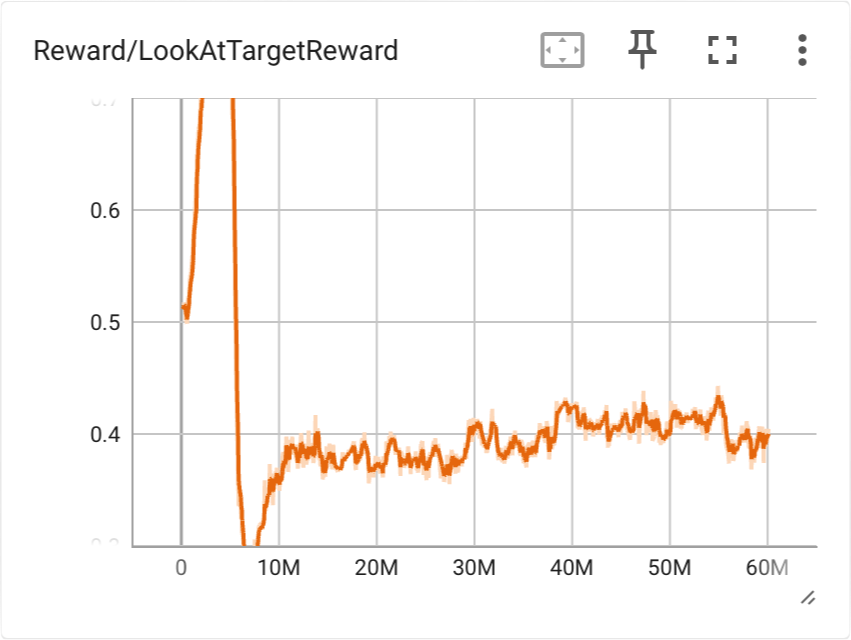
\includegraphics[width=\textwidth]{img/113_look_reward}
      \caption{Blickbelohnung}
      \label{fig:113_look_reward}
    \end{subfigure}
  \caption{Training Blickrichtungsziel mit Wechsel bei durchschnittlicher Blickbelohnung von 0.7}
  \label{fig:training_blickrichtungsziel_wechsel_07}
\end{figure}

Der Läufer braucht zu beginn eine ganze Weile um zu lernen sich bis zum Ziel zu bewegen. Aus diesem Grund verbringt der Läufer auch mit der neuen Bedingung zum erreichen des Blickziels zu viel Zeil des Trainings mit gleichbleibenden Blickzielwinkeln. Um von Anfang an und seperat vom erlernen des Laufens die Blickbelohnung zu erlernen, wird die Bedingung für das Erreichen eines Blickziels erneut angepasst. Im folgenden Versuch wird der Blickzielwinkel gewechselt sobald der Läufer 3 Sekunden auf das Ziel blickt. Implementiert wurde das ganze mit einem Spherecast um gleichzeitig zu ermöglichen die Genauigkeit mit der der Läufer auf das Ziel schauen muss anpassen zu können (siehe Abbildung \ref{fig:spherecast}).

\begin{figure}[H]
  \centering  
  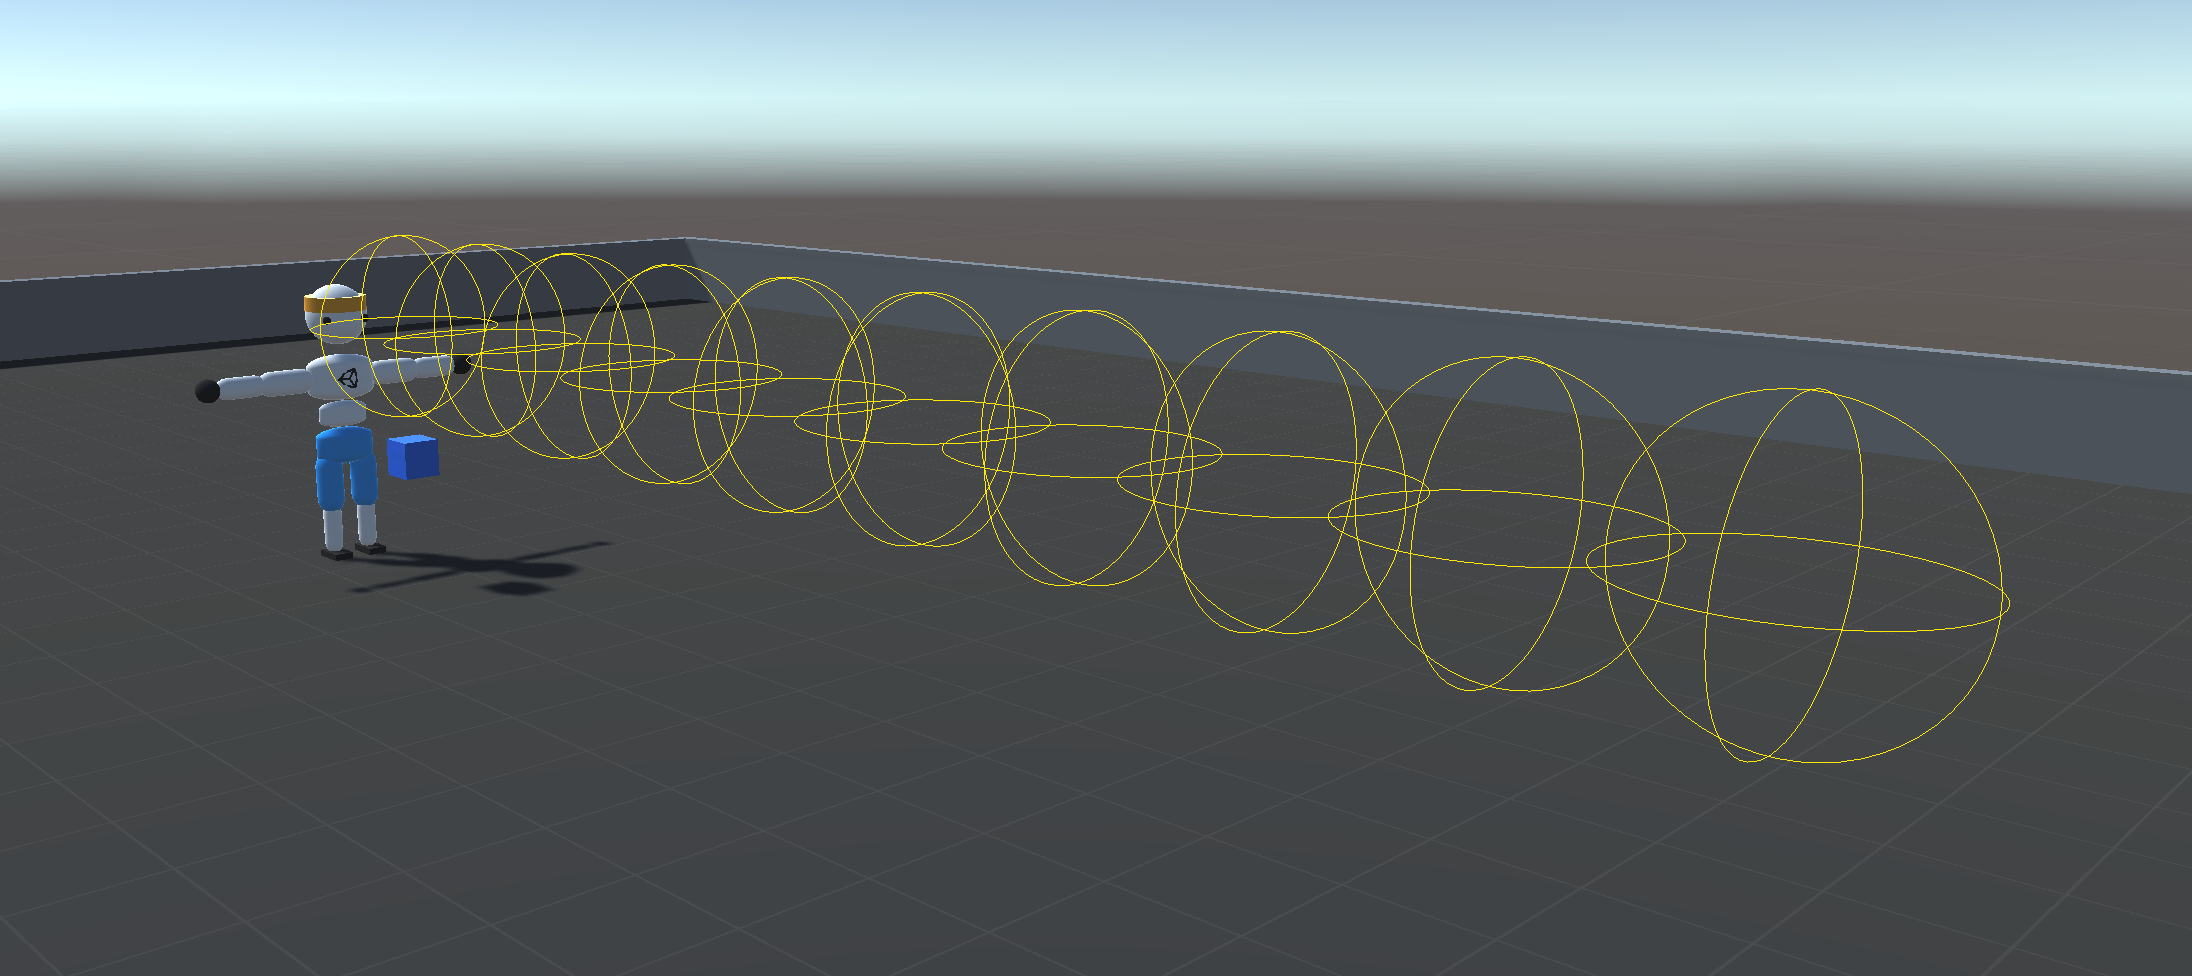
\includegraphics[width=0.8\textwidth]{img/spherecast}
  \caption{Blick Spherecast}
  \label{fig:spherecast}
\end{figure}

Ziel wird neu gesetzt wenn Läufer 3 sek auf das Ziel schaut (mit spherecast). (Schaut zuverlässig zu Ziel aber lernt sehr langsam das Laufen) 117
Verringern der Look at Zeit auf 2 sek. (Lernt gut zu laufen aber Blickbelohnung fällt extrem ab, schaut nicht auf Ziel) 118 / 119
\input{04_02_03_separate_bewegungsabläufe}
\subsection{4 Laufrichtungen}

\subsubsection{Versuch 7}
Die Charaktersteuerung benötigt je nach Tastatureingabe eine der vier Bewegungsrichtungen. Der Unity ML-Agents Agent enthält eine Funktion zum wechseln des verwendeten Modells. Mit dieser Funktion wird in folgender Implementierung zwischen den Modellen aus Versuch 6 gewechselt um alle Bewegungsrichtungen mit einer Steuerung abzudecken. Zu Erwarten ist das die Bewegung in die einzelnen Richtungen funktioniert, der Läufer aber beim Wechsel zwischen den Modellen das Gleichgewicht nicht halten kann.

\begin{lstlisting}[caption={Laufrichtung Modell wechseln},captionpos=b,label={lst:laufrichtung_modell_wechsel}]
public override void FixedUpdate() {
    ...    
    agent.targetWalkingSpeed = 5f;
    if (inputVert != 0) //Tastatur Input Vor oder Zurück
    {
        // Vorwärts
        if (inputVert > 0)
        {
            agent.SetModel("Walker", modelForward);
        }
        else // Zurück
        {
            agent.SetModel("Walker", modelBackward);
        }
    }
    else if (inputHor != 0) // Links oder Rechts
    {
        if (inputHor > 0) // Rechts
        {
            agent.SetModel("Walker", modelRight);
        }
        else // Links
        {
            agent.SetModel("Walker", modelLeft);
        }
    }
    else //kein Input -> Auf der Stelle stehen
    {
        agent.targetWalkingSpeed = 0f;
        agent.SetModel("Walker", modelStanding);
    }
    ...
}
\end{lstlisting}

Wie angenommen funktioniert das Bewegen in eine konstante Richtung gut. Beim Wechsel zu einem anderen Modell fällt der Läufer ohne Ausnahme.

\subsubsection{Versuch 8}
In Versuch 8 wird die Möglichkeit geprüft, alle Bewegungsrichtungen in einem Modell anzulernen. Dafür wird zum Start eine zufällige Bewegungsrichtung für jeden Läufer ausgewählt, mit dem Ziel das die Läufer direkt mit unterschiedliche Bewegungsrichtungen trainieren. Das gleichzeitige trainieren mit mehreren Läufern und unterschiedlichen Gehrichtungen soll das erlernen einer generell gültigen Strategie fördern. Die Gehrichtung wechselt beim erreichen eines Ziels, damit soll erreicht werden das der Läufer das aktuelle Ziel mit ausgewählter Bewegungsrichtung vollständig erlernt. Durch das öftere erreichen von Zielen im Verlauf des Trainings wird aber auch gleichzeitig jede beliebige Kombination angelernt. Als Ausgleich in der Komplexität wird die Zielgeschwindigkeit für das ganze Training festgesetzt.

\begin{lstlisting}[caption={Laufrichtung zufällig zum Start und beim erreichen von Ziel},captionpos=b,label={lst:laufrichtung_wechsel_start_ziel}]
public Direction direction = Direction.Forward;
Direction[] directions;

public override void Initialize()
{
    ...
    directions = (Direction[])Enum.GetValues(typeof(Direction));
    SetRandomWalkDirection();
    onTouchedTarget.AddListener(SetRandomWalkDirection);
}

public void SetRandomWalkDirection()
{
    direction = directions[Random.Range(0, directions.Length)];
}

public override void CollectObservations(VectorSensor sensor)
    {
        ...
        sensor.AddObservation((float)direction);
    }
\end{lstlisting}

Codeausschnitt \ref{lst:laufrichtung_wechsel_start_ziel} erstellt beim Initialisieren des Agenten ein Array mit allen Werten, welche das Richtungs-Enum zulässt. Die Funktion SetRandomWalkDirection wählt eine zufällige Richtung aus und setzt diese für den Agenten. Die Funktion wird zu Beginn in Initialize aufgerufe. Zusätzlich wird die Methode mit einem Listener auf das onTouchedTarget des Agenten registriert. Die Methode wird somit bei jedem berühren eines Ziels ausgeführt. Das der Agent während dem Training sowie nach dem Training zwischen den Laufrichtungen entscheiden kann, bekommt er einen Zahlenwert repräsentativ für die Richtung in der Beobachtung angehängt.

Der Läufer lernt unter diesen Bedingungen sehr langsam und das Training stagniert. Ab ca. 20 millionen Trainingsschritten fängt der Läufer an regelmäßig Ziele zu erreichen. Durch das häufige erreichen von Zielen steigt aber auch die Anzahl der Ziel- und Laufrichtungswechsel. Aus diesem Grund brechen die Belohnungen ein und der Fortschritt stagniert (siehe Abbildung \ref{fig:versuch8_training}).

\begin{figure}[H]
  \centering  
  \begin{subfigure}{.49\textwidth}
      \centering  
      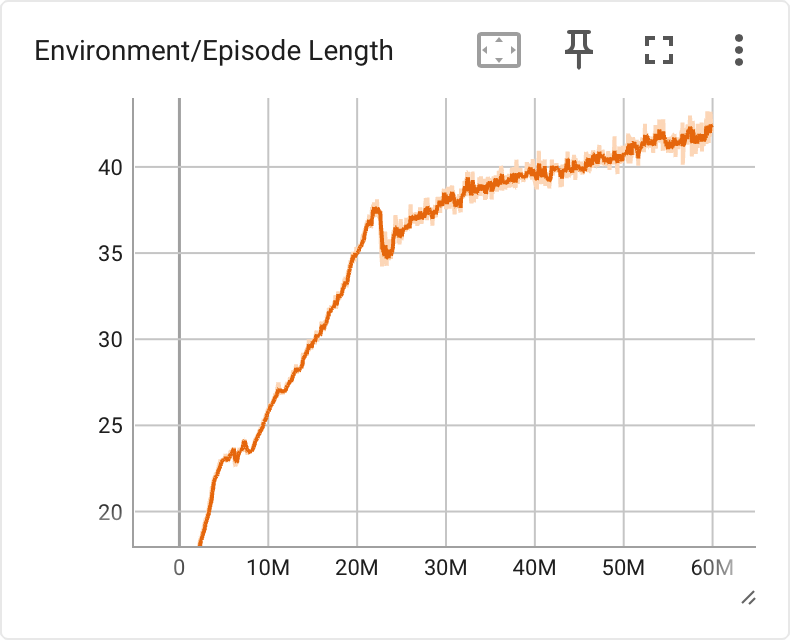
\includegraphics[width=\textwidth]{img/134_episode_length}
      \caption{Episodenlänge}
      \label{fig:134_episode_length}
    \end{subfigure}
    \begin{subfigure}{.49\textwidth}
      \centering  
      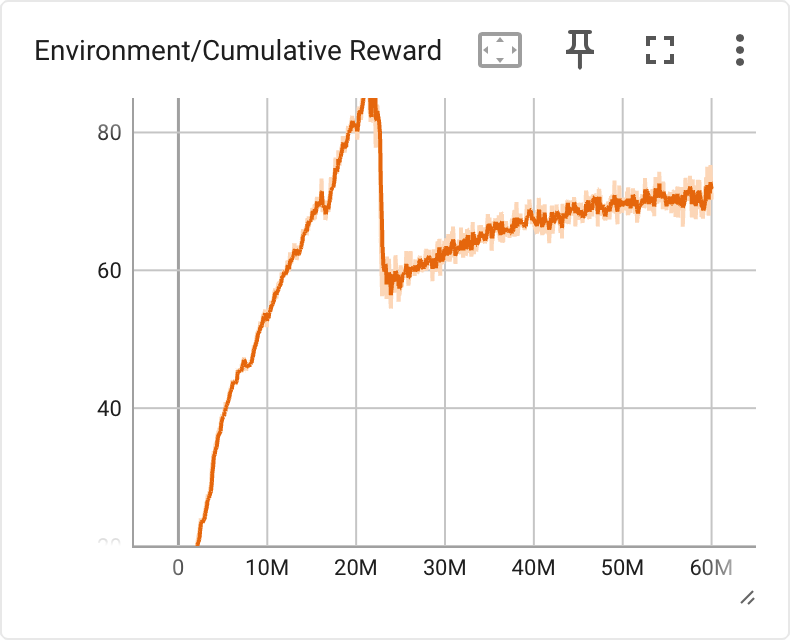
\includegraphics[width=\textwidth]{img/134_cumulative_reward}
      \caption{Angehäufte Belohnung}
      \label{fig:134_cumulative_reward}
    \end{subfigure}
     \begin{subfigure}{.49\textwidth}
      \centering  
      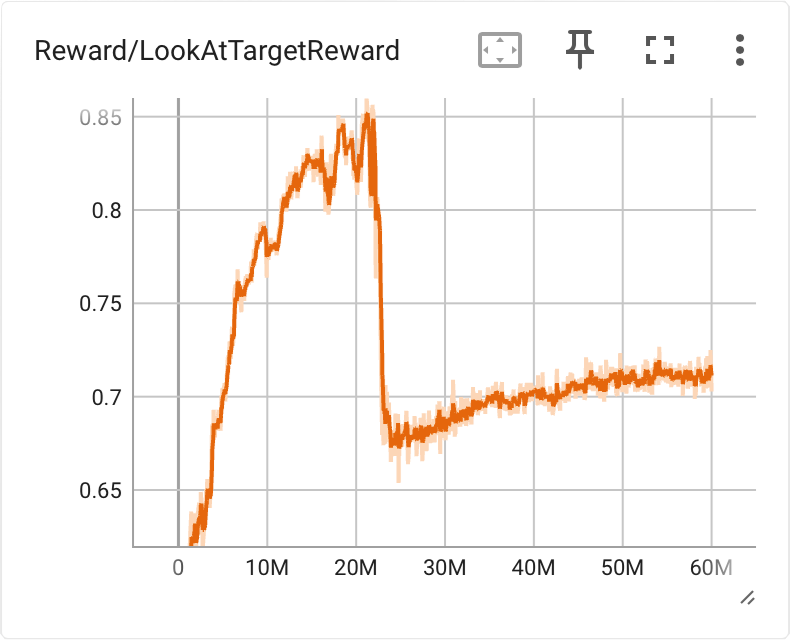
\includegraphics[width=\textwidth]{img/134_look_reward}
      \caption{Blickbelohnung}
      \label{fig:134_look_reward}
    \end{subfigure}
    \begin{subfigure}{.49\textwidth}
      \centering  
      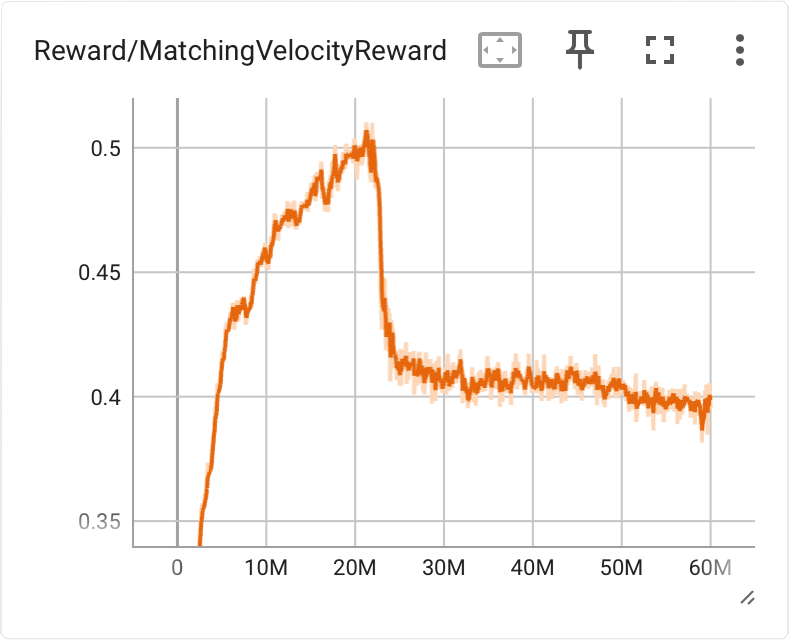
\includegraphics[width=\textwidth]{img/134_vel_reward}
      \caption{Geschwindigkeitsbelohnung}
      \label{fig:134_vel_reward}
    \end{subfigure}
    \begin{subfigure}{.49\textwidth}
      \centering  
      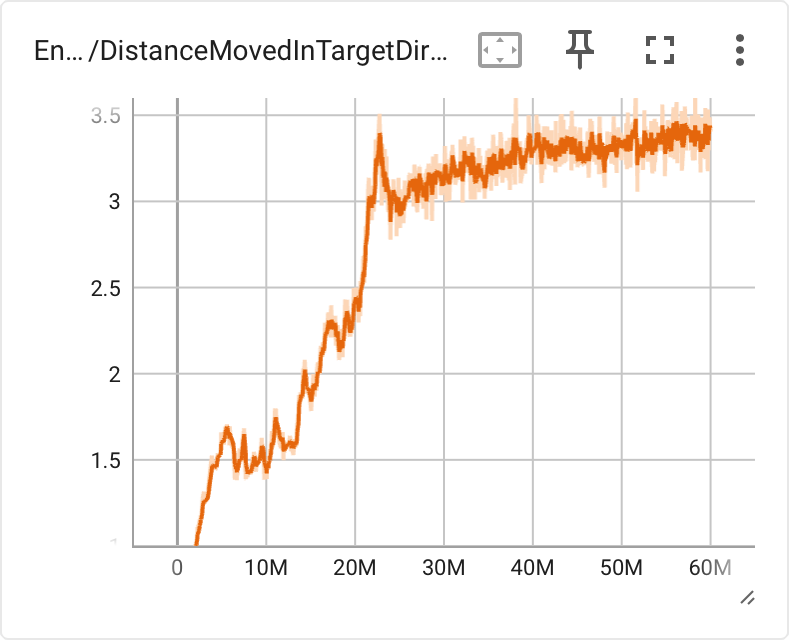
\includegraphics[width=\textwidth]{img/134_move_target_dir}
      \caption{Zurückgelegte Stecke in Zielrichtung}
      \label{fig:134_move_target_dir}
    \end{subfigure}
    \begin{subfigure}{.49\textwidth}
      \centering  
      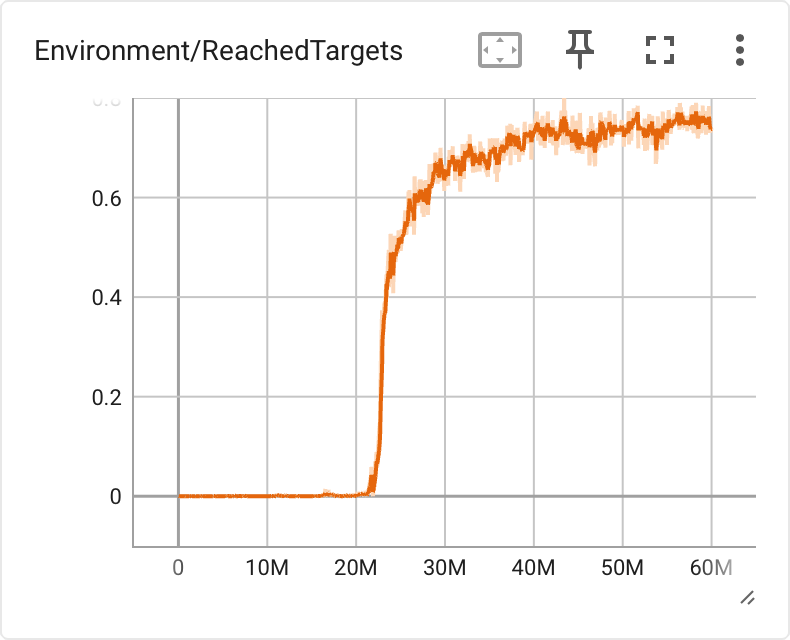
\includegraphics[width=\textwidth]{img/134_reach_target}
      \caption{Anzahl erreichte Ziele}
      \label{fig:134_reach_target}
    \end{subfigure}
  \caption{Versuch 8 Training Graphen}
  \label{fig:versuch8_training}
\end{figure}

\subsubsection{Versuch 9}
Um den Richtungswechsel regelmäßiger zu gestalten, wird getestet wie das Training sich verhält wenn die Richtung beim Start jeder neuen Trainingsepisode zufällig gewählt wird.

\begin{figure}[H]
  \centering  
  \begin{subfigure}{.49\textwidth}
      \centering  
      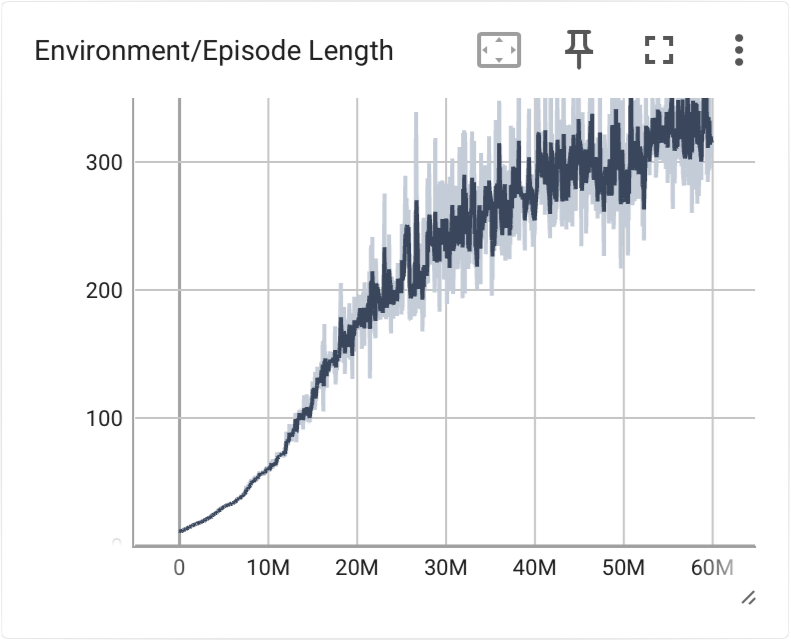
\includegraphics[width=\textwidth]{img/135_episode_length}
      \caption{Episodenlänge}
      \label{fig:135_episode_length}
    \end{subfigure}
    \begin{subfigure}{.49\textwidth}
      \centering  
      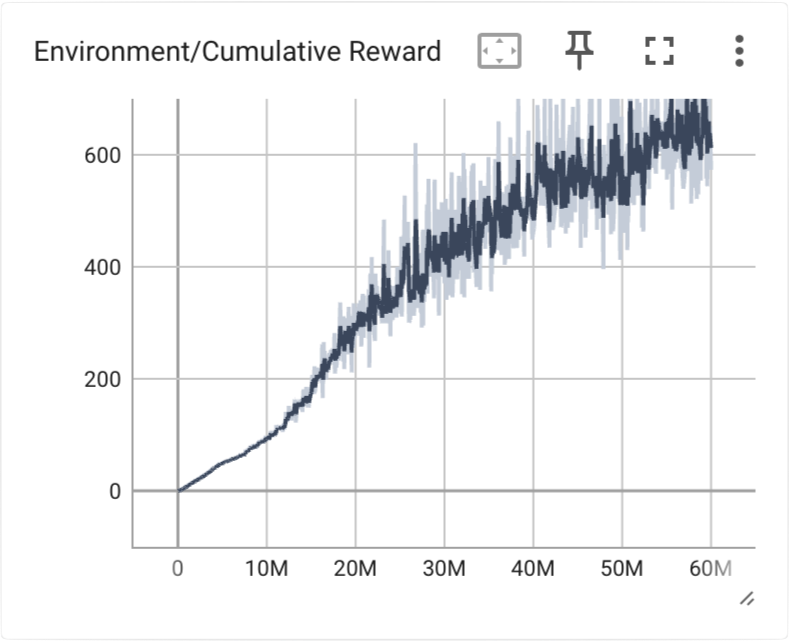
\includegraphics[width=\textwidth]{img/135_cumulative_reward}
      \caption{Angehäufte Belohnung}
      \label{fig:135_cumulative_reward}
    \end{subfigure}
     \begin{subfigure}{.49\textwidth}
      \centering  
      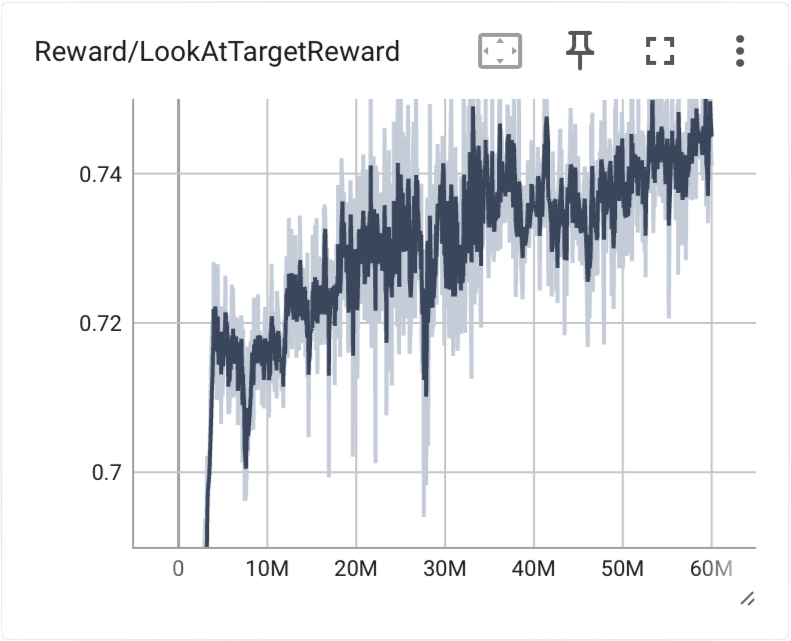
\includegraphics[width=\textwidth]{img/135_look_reward}
      \caption{Blickbelohnung}
      \label{fig:135_look_reward}
    \end{subfigure}
    \begin{subfigure}{.49\textwidth}
      \centering  
      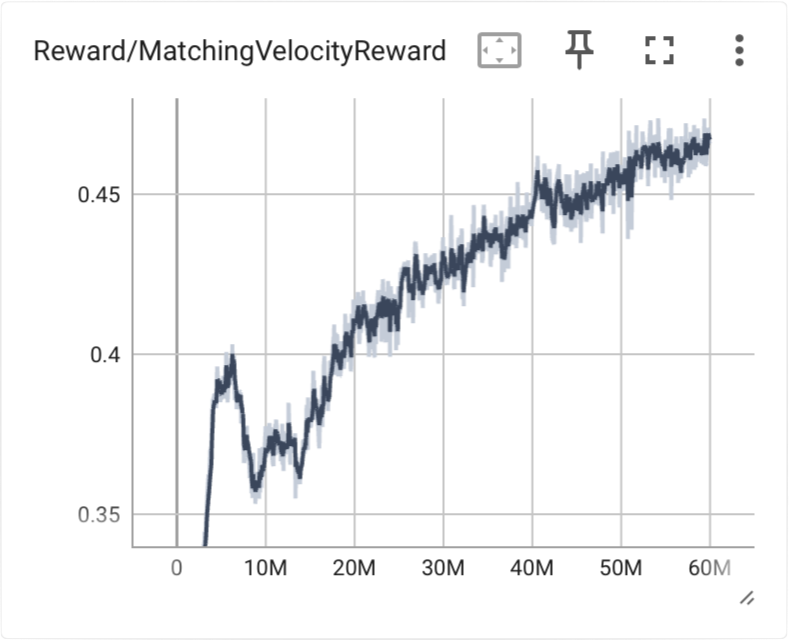
\includegraphics[width=\textwidth]{img/135_vel_reward}
      \caption{Geschwindigkeitsbelohnung}
      \label{fig:135_vel_reward}
    \end{subfigure}
    \begin{subfigure}{.49\textwidth}
      \centering  
      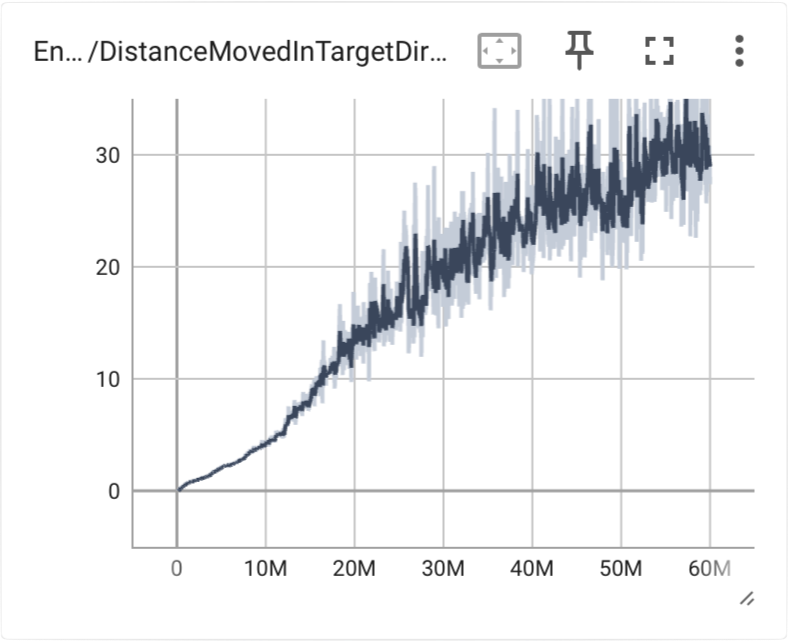
\includegraphics[width=\textwidth]{img/135_move_target_dir}
      \caption{Zurückgelegte Stecke in Zielrichtung}
      \label{fig:135_move_target_dir}
    \end{subfigure}
    \begin{subfigure}{.49\textwidth}
      \centering  
      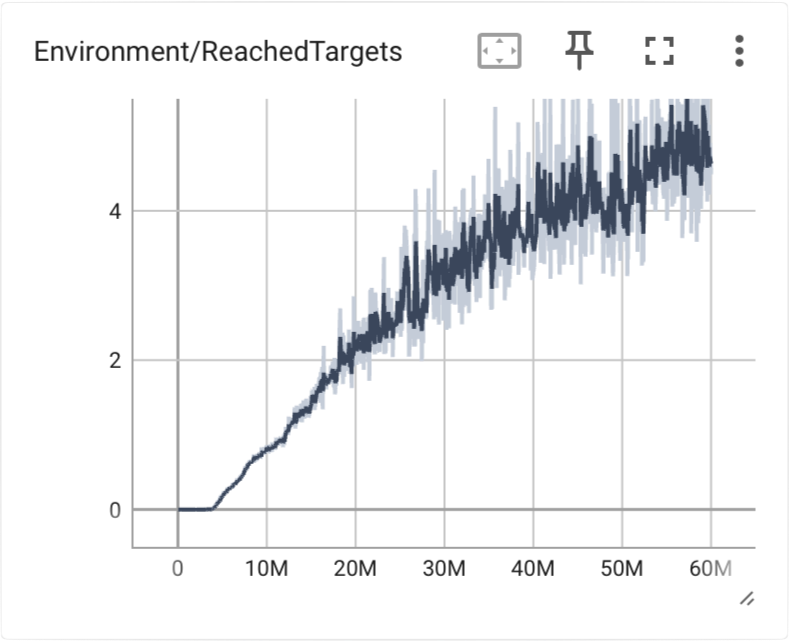
\includegraphics[width=\textwidth]{img/135_reach_target}
      \caption{Anzahl erreichte Ziele}
      \label{fig:135_reach_target}
    \end{subfigure}
  \caption{Versuch 9 Training Graphen}
  \label{fig:versuch9_training}
\end{figure}

Das gleichbleiben der Laufbewegung über die komplette Trainingsepisode hat zur folge dass das Training stabiler verläuft siehe Abbildung \ref{fig:versuch9_training}. Der Nachteil ist jedoch das der Läufer keine Bewegungswechsel lernt. Beim steuern des Läufers ist das wechseln zwischen den Laufrichtungen noch immer ein Problem. Dazu kommt das der in diesem training die Blickrichtungs Belohnung geringer ist als bei vorherigen Trainingseinheiten. Der Läufer lernt die seitwärts Bewegungen nicht richtig sondern nimmt einen Verlust in der Belohnung in kauf für die Steigerung der Episodenlänge.